% ***********************************************************
% ******************* PHYSICS HEADER ************************
% ***********************************************************
% Version 2
\documentclass[11pt]{article} 
\usepackage{amsmath} % AMS Math Package
\usepackage{amsthm} % Theorem Formatting
\usepackage{amssymb}	% Math symbols such as \mathbb
\usepackage{graphicx} % Allows for eps images
\usepackage{multicol} % Allows for multiple columns
\usepackage[dvips]{geometry}
 % Sets margins and page size
\pagestyle{empty} % Removes page numbers
\makeatletter % Need for anything that contains an @ command 
\renewcommand{\maketitle} % Redefine maketitle to conserve space
{ \begingroup \vskip 10pt \begin{center} \large {\bf \@title}
	\vskip 10pt \large \@author \hskip 20pt \@date \end{center}
  \vskip 10pt \endgroup \setcounter{footnote}{0} }
\makeatother % End of region containing @ commands
\renewcommand{\labelenumi}{(\alph{enumi})} % Use letters for enumerate
% \DeclareMathOperator{\Sample}{Sample}
\let\vaccent=\v % rename builtin command \v{} to \vaccent{}
\renewcommand{\v}[1]{\ensuremath{\mathbf{#1}}} % for vectors
\newcommand{\gv}[1]{\ensuremath{\mbox{\boldmath$ #1 $}}} 
% for vectors of Greek letters
\newcommand{\uv}[1]{\ensuremath{\mathbf{\hat{#1}}}} % for unit vector
\newcommand{\abs}[1]{\left| #1 \right|} % for absolute value
\newcommand{\avg}[1]{\left< #1 \right>} % for average
\let\underdot=\d % rename builtin command \d{} to \underdot{}
\renewcommand{\d}[2]{\frac{d #1}{d #2}} % for derivatives
\newcommand{\dd}[2]{\frac{d^2 #1}{d #2^2}} % for double derivatives
\newcommand{\pd}[2]{\frac{\partial #1}{\partial #2}} 
% for partial derivatives
\newcommand{\pdd}[2]{\frac{\partial^2 #1}{\partial #2^2}} 
% for double partial derivatives
\newcommand{\pdc}[3]{\left( \frac{\partial #1}{\partial #2}
 \right)_{#3}} % for thermodynamic partial derivatives
\newcommand{\ket}[1]{\left| #1 \right>} % for Dirac bras
\newcommand{\bra}[1]{\left< #1 \right|} % for Dirac kets
\newcommand{\braket}[2]{\left< #1 \vphantom{#2} \right|
 \left. #2 \vphantom{#1} \right>} % for Dirac brackets
\newcommand{\matrixel}[3]{\left< #1 \vphantom{#2#3} \right|
 #2 \left| #3 \vphantom{#1#2} \right>} % for Dirac matrix elements
\newcommand{\grad}[1]{\gv{\nabla} #1} % for gradient
\let\divsymb=\div % rename builtin command \div to \divsymb
\renewcommand{\div}[1]{\gv{\nabla} \cdot #1} % for divergence
\newcommand{\curl}[1]{\gv{\nabla} \times #1} % for curl
\let\baraccent=\= % rename builtin command \= to \baraccent
\renewcommand{\=}[1]{\stackrel{#1}{=}} % for putting numbers above =
\newtheorem{prop}{Proposition}
\newtheorem{thm}{Theorem}[section]
\newtheorem{lem}[thm]{Lemma}
\theoremstyle{definition}
\newtheorem{dfn}{Definition}
\theoremstyle{remark}
\newtheorem*{rmk}{Remark}

% ***********************************************************
% ********************** END HEADER *************************
% ***********************************************************

%%% Local Variables:
%%% mode: latex
%%% TeX-Master: notes
%%% End:

\usepackage[utf8]{inputenc}
\usepackage{amsmath}
\usepackage{amssymb}
\usepackage{amsfonts}
\usepackage{amssymb}
\usepackage{float}
\usepackage{indentfirst}
\usepackage{vmargin}
\usepackage{indentfirst}
\usepackage{titling}
\usepackage{color} 
\usepackage{siunitx}
\usepackage{xspace}
\usepackage{graphicx}
\usepackage{enumitem}
\usepackage[backend=biber,backref=true,style=unsrt,
style=numeric-comp,block=ragged,firstinits=true]{biblatex}
\addbibresource{ref-notes.bib}
\bibliography{ref-notes}
\graphicspath{{plot_synthesis/} {Feynman/}}

\newcommand{\mastersig}{\ensuremath{\Im{\widehat{\Sigma}^{A,B}(k,E)}}\xspace}
\newcommand{\chiqw}{\ensuremath{\Im{\chi}(q,\omega)}\xspace}

\providecommand{\norm}[1]{\lVert#1\rVert}

\newcommand{\subtitle}[1]{%
  \posttitle{%
    \par\end{center}
    \begin{center}\large#1\end{center}
    \vskip0.5em}%
}


\title{Condensed Matter II}
\subtitle{Problem set \#5}
%\author{}
\date{Spring 2014}

\begin{document}

\maketitle

\setlength{\unitlength}{1cm}
%\advance\textwidth by 3cm
%\advance\hoffset by -1.5cm 
\advance\textheight by 1cm
\advance\voffset by -1.5cm
\setmarginsrb{3cm}{0.5cm}{1.5cm}{1cm}{1cm}{1cm}{1cm}{1cm}
%\setlength{\parindent}{0cm}%

\pagestyle{plain}

\section{Density of states of Si, Ge, Sn}

\begin{figure}[h]
  \centering
  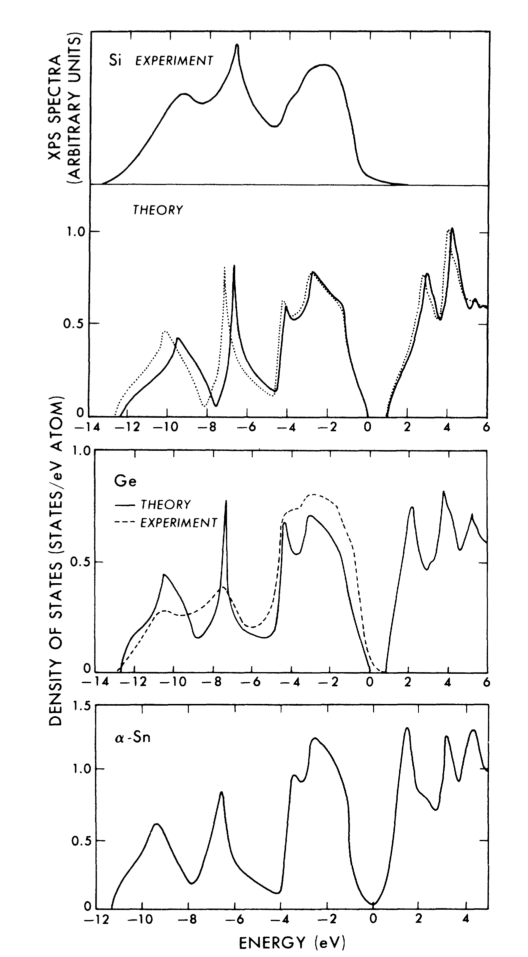
\includegraphics[width=9cm]{DOS_SiGeSn.pdf}
  \caption{Calculated electronic densities of states compared to
    experiment for Si, Ge, and $\alpha$-Sn. The experimental results
    for Si and Ge are from Pollak et al., PRL 29, 1103 (1973) and
    Grobman et al., PRL 29, 1508 (1972) respectively. In the case of Si, two results are
    displayed: nonlocal pseudopotential (solid line) and local
    pseudopotential (dashed line). R. Chelikowsky et al., PRB 14, 556 (1976)\label{fig:dos}}
\end{figure}


Based on the density of states of Si, Ge, and $\alpha$-Sn displayed
in Fig~\ref{fig:dos}, comment on the density of states of the empty
diamond lattice (assuming isotropic effective mass $m_0$ and lowest
energy point of the density of states at $E_0$=-13eV). Where is the
Fermi energy located in this model?

\section{Study of ReO$_3$}

The electronic structure of Re is $4f^{14}5d^56s^2$, that of O is
$2s^22p^4$. The band structure of ReO$_3$ is displayed in
Fig~\ref{fig:band_reo3}, and its unit cell and Brillouin zone are
displayed in Fig~\ref{fig:BZreo3}

\begin{figure}[h]
  \centering
  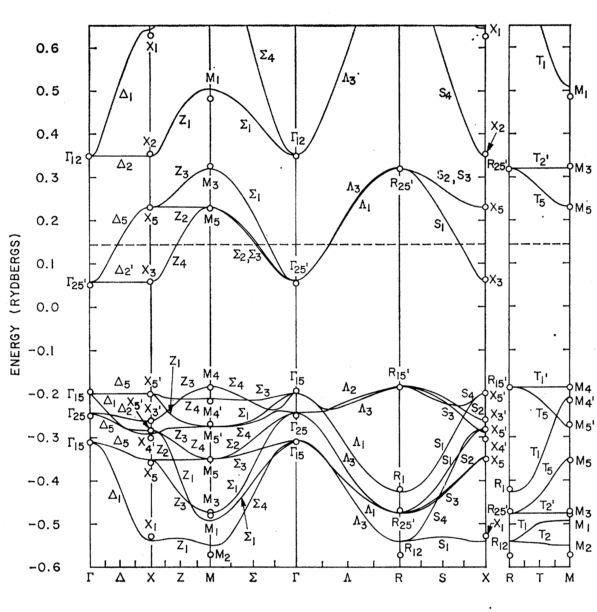
\includegraphics[width=16cm]{reo3_bands_v2.pdf}
  \caption{Tight-binding energy bands for ReO$_3$ obtained by fitting
    APW results at symmetry points.  Mattheiss, Physical Review
    181, 987 (1969)\label{fig:band_reo3}}
\end{figure}


\begin{figure}[h]
  \centering
  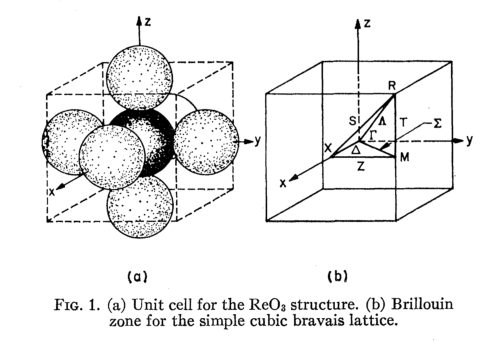
\includegraphics[width=12cm]{reo3bz.pdf}
  \caption{(a) Unit cell for the ReO$_3$ structure. (b) Brillouin zone
    for the simple cubic bravais lattice. Mattheiss, Physical Review
    181, 987 (1969)\label{fig:BZreo3}}
\end{figure}

\begin{enumerate}[label=(\roman*)]
\item How many atoms per unit cell does the structure count?
\item Which are the Re energy bands, which are the O energy bands?
\item Is ReO$_3$ a metal, or a semiconductor?
\item Identify the d-bands on Fig~\ref{fig:band_reo3}. To which of the Re
  or O atom are they associated? Where are the other atom's d-bands
  located?
\item Identify the location of the carrier pockets, and qualitatively assess the
  effective masses of the carriers.
\item Assess the number of electrons per carrier pocket.
\item Where does the lowest energy optical transition occur? Comment
  on its expected strength.
\end{enumerate}

%\section

\end{document}